\chapter{LIME}\label{ch:lime}

A LIME egy modell-agnosztikus magyarázatgeneráló rendszer. A LIME feloldása \foreignlanguage{english}{Linear Model-Agnostic Expalantions}, melyben a lineáris arra referál, hogy egy lineáris modell a magyarázat. A keretrendszer képes szöveg, kép és egyszerű egy dimenziós vektorként megadott tulajdonságokkal dolgozó modellek magyarázatára. 

\section{Az ideális magyarázó elvárásai}

Legyen most a magyarázatgenerálás célja a tanító adathalmazbeli zajok által létrehozott rossz általánosítás eredményező modell karakterisztikák egyszerűen felismerhetővé tétele. Nem csak a probléma létének felismerése, hanem forrásának beazonosítása is cél, azokban az esetekben is, mikor a probléma nem okoz helytelen kimenetet.

Az egyszerű felismerhetőség egzakt módon nehezen megfogható koncepció. A minimum hogy a területben járatos szakemberek egy magyarázat alapján a modell a példa körüli lokális működésének helyességét viszonylagos biztossággal meg tudják ítélni rövid idő alatt. Hogy a magyarázatok reprezentatívak legyenek a teljes modellre nézve, sok magyarázat kiértékelésére van szükség, ezért a gyors értékelhetőség igénye kritikus fontosságú. A legjobb eredmény eléréséhez kompromisszumra van szükség a magyarázat komplexitása és a kiértékelés időigénye közt.

A LIME rendszer a magyarázatokra intuitív működésük és egyszerűségük miatt lineáris modelleket használ, ezen túl a kiértékelendő magyarázatok számának csökkentése érdekében a submodular pick algoritmust használja.

\section{Lokális magyarázatok}

Egy komplex nem-lineáris modell működése globálisan nem közelíthető egy lineáris modell segítségével, mivel az csak lineárisan szerparálható feladatokat képes megoldani, ahogy az \aref{sec:linszep} szekcióban tárgyalva volt. Viszont az állapottér egy kisebb részét tekintve egy lineáris modell is reprezentatív lehet, ez a lokális közelítés. A lokalitás eléréséhez a lime két módszer kombinációját alkalmazza:

%TODO mekkkora környezetben véges mintavételt?
%a scikit random normal az normál eloszlást csinál?
\begin{itemize}
	\item a magyarázandó példa körül véletlen mintavételezés
	\item a hibafüggvény súlyozása egy $\pi_x (z)$ távolságfüggvénnyel
\end{itemize}

A folytonos tulajdonságok mintavételezése normál eloszlás alapú véletlen számmal történik, aminek értékét a tanító adathalmazból meghatározott értékkészlettel skáláz a rendszer. A kategorikus tulajdonságok esetében pedig a tanító adathalmazból kiszámolt gyakoriságok alapján generált véletlen kategóriával történik. A magyarázandó példát mindig tartalmazza mintavételezéssel létrehozott adathalmazhoz.

A a távolsághoz képest vett súlyozás függvénye

\begin{equation}
    \pi_x (z) = exp\left(\frac{-D(x',z')^2}{\sigma^2}\right),
\end{equation}

ahol $x'$ a magyarázandó példa, $z'$ az $x'$ körüli generált példa, $D$ egy távolságfüggvény ami alkalmazási területenként változhat. Például szövegek esetén koszinusz távolság, képek esetén euklideszi távolság. $\sigma$ pedig egy szélességi paraméter ami megadja, hogy az eseménytér mekkora hányadát fedje le a $\pi$ függvény. $\sigma$ érték alapértelmezetten $|\x'|*0.75$ ($|\x'|$ a bemeneti tulajdonságok száma), de explicit módon is megadható.

\begin{figure}[H]
    \centering
		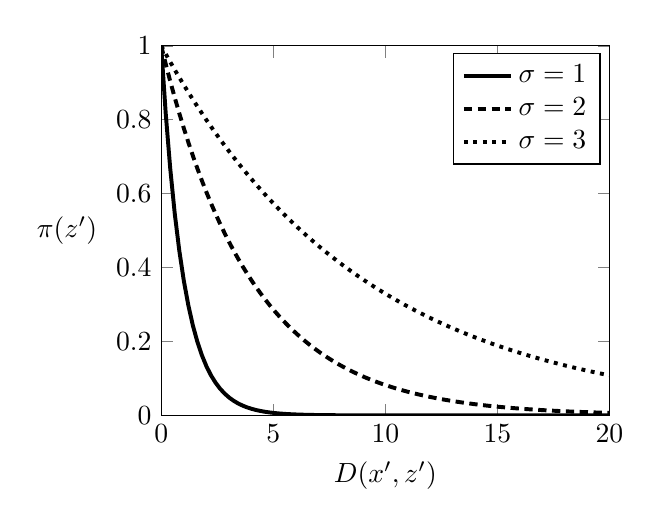
\begin{tikzpicture}
            \begin{axis} [width=0.6\textwidth,samples=100,xmin=0,xmax=20,xlabel={$D(x',z')$}, ylabel={$\pi(z')$},ylabel style={rotate=-90},ymin=0, ymax=1,domain=0:20, legend entries =  {$\sigma = 1$\\$\sigma=2$\\$\sigma=3$\\},]
                \addplot[mark=none,line width=0.5mm] {e^(-x/1)};
                \addplot[mark=none,densely dashed,line width=0.5mm] {e^(-x/4)};
                \addplot[mark=none,dotted,line width=0.5mm] {e^(-x/9)};
                %\node at (-1.5,0.75) {$f(x) = \cfrac{1}{1+e^{-x}}$};
            \end{axis}
        \end{tikzpicture}
	\caption{Példák súlyozása a magyarázandó példától vett távolság függvényében, három különböző szigma értékre}
\end{figure}

Maga a $g(z')$ magyarázat modell tehát így néz ki:

\begin{equation}
    g(z') = w_g\cdot z'
\end{equation}

és az optimalizálandó hibafüggvény:

\begin{equation}
    L(y,g,\pi_x) = \sum_{z' \in \boldysmbol Z} \pi_x(z')\left(y(z')-g(z')\right)^2 
\end{equation}


\subsection{Értelmezhetőség}

Egy lineáris modell önmagában egyszerűen értelmezhető még laikusok számára is, mivel a menetekhez tartozó súly értelmezhető a tulajdonság fontosságaként. A negatív súlyú tulajdonságok azt is megadják, hogy mely változók jelenléte csökkenti a modell bizonyosságát a prediktált osztályban.

Viszont nagyszámú attribútum esetén egy lineáris modell sem értelmezhető egyszerűen. Nem elvárható, hogy a felhasználó például 1000 paramétert végignézzen. Ráadásul nagy számú paraméter esetén a túltanulás veszélye lineáris modellek esetén is megnő.
Ennek elkerülése végett érdemes maximalizálni a magyarázat által felhasznált tulajdonságok számát, legyen ez a felső korlát $K$. $K$ értéke nem lehet nagyon kicsi, mert fontos tulajdonságok maradhatnak ki, de túl nagy sem lehet, mert az nagyon lassítaná a kiértékelési procedúrát. Ökölszabályként használható a a $K=7-8$ érték, mivel becslések alapján ennyi független dolgot képes az agy egyidőben a rövidtávú memóriában tárolni. 

Erre a problémára a lime több alternatív megoldást is kínál:
\begin{itemize}
    \item iteratív módon hozzáadni a modellt leginkább javító tulajdonságokat
    \item a legnagyobb súlyú értékek választása
    \item LASSO regularizáció
\end{itemize}

Az iteratív kiválasztás minőségi eredményt szolgáltat, de nagyon költséges. Minden tulajdonság hozzáadásánál az összes fennmaradó tulajdonságra be kell tanítani egy modellt, ami $|x| >> K$ esetben közelítőleg $K*|x|$ tanítási folyamatot jelent. Költsége miatt automatikus esetben a LIME $K<6$ esetben használja ezen módszert. 

A legmagasabb súly kiválasztásán alapuló módszer esetén egy modellt tanít a rendszer, majd a súlyokat megszorozza a magyarázandó példa tulajdonságaival, az így kapott értékek közül a K legnagyobbat használja fel a magyarázatban. Ez a módszer nagyon gyors, viszont nem véd a túltanulás ellen. Például egy olyan esetben, ahol bináris tulajdonságok vannak és van egy tulajdonság ami a mintákban csak kevés esetben vesz fel 1 értéket, de az esetben a célváltozó is mindig aktív, ezért a modell nagy súlyt fog hozzárendelni, pedig nem feltétlenül fontos változó. 

A LASSO módszer regularizáció segítségével választja ki a magyarázatba bekerülő tulajdonságokat. A módszer lényege, hogy a felhasznált súlyok abszolútérték-összege növekedését bünteti azzal, hogy egy $\alpha$ skalárral megszorozva hozzáadja a hibafüggvényhez. A LIME rendszer a least angle regression algoritmust használja a LASSO regularizált modell számításához.

\section{Magyarázandó példák kiválasztása}

Véletlenszerűen kiválasztott példák esetén redundánsak lehetnek a magyarázatok. Két magyarázat akkor redundáns, ha azonos okokból történik a predikció, azaz a magyarázatban ugyanazok az attribútumok szerepelnek hasonló súlyokkal. 

A redundancia elkerülésére a LIME a submodular pick algoritmust alkalmazza. Az algoritmus felhasznál egy már létrehozott magyarázat halmazt, mely optimális esetben tartalmazza az összes rendelkezésre álló példa magyarázatát. Ezen példákba beletartoznak a tanító példák is, amik bár pontosság meghatározására túltanulás miatt nem használhatóak, de magyarázatok esetén pont hogy hasznos hogy felszínre hozza a túltanulásból adódó problémákat. Ez az ideális eset futási idő szempontjából gyakran nem elérhető és ha az is, lehetséges hogy egy kisebb számú magyarázatot de jobb minőséget adó algoritmus előnyösebb.

\newcommand{\W}{\ensuremath{\boldsymbol W}}

Legyen \W a magyarázatok mátrixa, melyben minden oszlop egy tulajdonsághoz tartozik, a sorok pedig a magyarázatokhoz. Legyen \W minden eleme nulla, majd a magyarázatokban szereplő tulajdonságokhoz tartozó elemeket állítsuk a hozzá tartozó súly abszolút értékére. Egy tulajdonság jelentőségét jelölje $I$, értéke pedig legyen

\begin{equation}
    I_{j} = \sqrt{\sum_{i=1}^{n} \W_{i,j}}
\end{equation}

Minél nagyobb $I$ érték tartozik egy tulajdonsághoz az algoritmus annál fontosabbnak tartja, hogy azt tartalmazó példa bekerüljön a szűrt magyarázat listába.

Az algoritmus mohó módon kiválasztja azt a magyarázatot, melyben szereplő tulajdonságok $I$ szummája maximális. Ezután a kiválasztott magyarázat tulajdonságainak $I$ értékét nullára állítja, mivel hozzáadott értékkel nem jár ha kétszer is bekerülnek, mivel az redundáns lenne.

Ezen lépésnél van jelentősége annak is, hogy $I$ értéke gyökös, mivel így két kisebb jelentőségű tulajdonság bevételét fontosabbnak tartja az algoritmus, mint egy a másikét ami kétszer fontosabb. Ezáltal több különböző tulajdonság szerepelhet a szűrt listában.

A submodular pick gyors futási időt biztosít de elhanyagol pár tényezőt. Lehetséges, hogy a legfontosabb tényezőkből érdemes szándékosan többet is bevenni, hogy a kiértékelő számára egyértelműbb legyen a tulajdonság fontossága. Természetesen bekerülhet egy tulajdonság több különböző magyarázatba is, de csak akkor ha az a példa más tulajdonság miatt lett kiválasztva. 

Ezen kívül ha már minden tulajdonság bekerült a szűrt halmazba, az algoritmus nem képes több magyarázatot kiválasztani. Ez természetesen egyszerűen orvosolható például az algoritmus újrafuttatásával, ahol a már kiválasztott magyarázatok kikerülnek a bemenetből.

